
\documentclass[mctitle,oldtoc,a4paper,11pt,oneside]{sty/topspinrapport}

\usepackage[margin=1.0in]{geometry}

\font\chapterfont=cmssdc10 at 40pt
\font\secfont=cmssdc10 at 14pt
\font\ssecfont=cmssdc10 at 12pt
\font\problemfont=cmssdc10 at 14pt
%

\HeadingFonts{\bfseries}{\bfseries}{\chapterfont}{\secfont}{\ssecfont}{\slshape}{\slshape}{\slshape}



%\usepackage{mathpazo}

\usepackage{graphicx}
\usepackage{amssymb,amsmath}
\usepackage{latexsym}
\usepackage{nopageno}
\usepackage{listings}
\usepackage{times}


%%%%%%%%%%%%%%%%%%%%%%
% Referencing macros %
%%%%%%%%%%%%%%%%%%%%%%

\newcommand{\figref}[1]{Figure~\ref{fig:#1}}


%%%%%%%%%%%%%%%%%%
% Listings stuff %
%%%%%%%%%%%%%%%%%%

\newcommand{\inline}[1]
{\lstset{
basicstyle=\footnotesize\tt}\lstinline|#1|\lstset{
basicstyle=\scriptsize\tt}}

\lstset{
basicstyle=\scriptsize\tt,
commentstyle=\footnotesize\tt, aboveskip=\medskipamount,
belowskip=\medskipamount, xleftmargin=0pt, captionpos=b}


%%%%%%%%%%%%%%%%%%
% Names of tools %
%%%%%%%%%%%%%%%%%%

\newcommand{\etch}{\mbox{E\scalebox{0.75}{TCH}}}
\newcommand{\gap}{\mbox{G\scalebox{0.75}{AP}}}
\newcommand{\spin}{\mbox{S\scalebox{0.75}{PIN}}}
\newcommand{\topspin}{\mbox{TopS\scalebox{0.75}{PIN}}}
\newcommand{\saucy}{{\it saucy}}
\newcommand{\symmextractor}{SymmExtractor}
\newcommand{\symmreducer}{SymmReducer}
\newcommand{\gcc}{GCC}


%%%%%%%%%%%%%%%%%%
% URLs           %
%%%%%%%%%%%%%%%%%%

\newcommand{\topspinwebpage}{http://www.allydonaldson.co.uk/topspin/}
\newcommand{\sourceforgepage}{https://www.sourceforge.net/projects/symmetryglasgow/}
\newcommand{\sableccwebsite}{http://sablecc.org/}
\newcommand{\saucywebpage}{http://vlsicad.eecs.umich.edu/BK/SAUCY/}
\newcommand{\winrarwebsite}{http://www.rarlab.com/}
\newcommand{\javaurl}{http://java.sun.com/}
\newcommand{\spinurl}{http://www.spinroot.com/}
\newcommand{\gapurl}{http://gap-system.org/}
\newcommand{\gccurl}{http://gcc.gnu.org/}


%%%%%%%%%%%%%%%%%%
% Useful macros  %
%%%%%%%%%%%%%%%%%%

\newcommand{\chapref}[1]{Chapter~\ref{chapter:#1}}
\newcommand{\chapsref}[2]{Chapters~\ref{chapter:#1} and~\ref{chapter:#2}}
\newcommand{\secref}[1]{\S\ref{sec:#1}}

\newcommand{\seesec}[1]{see \secref{#1}}

\newcommand{\problem}[1]{\noindent{\bf Problem:} #1}
\newcommand{\solution}[1]{\noindent{\bf Solution:} #1}
\newcommand{\exampleerrormessage}{\vspace{1mm}\noindent{\bf Example error message:}}

\newcommand{\ltl}{$\mathit{LTL}$}

%%%%%%%%%%%%%%%%%%
% Versions       %
%%%%%%%%%%%%%%%%%%

\newcommand{\sableccversion}{3.2}
\newcommand{\topspinversion}{2.2}
\newcommand{\jreversion}{1.5.0\_06}
\newcommand{\gccversion}{3.4.4}
\newcommand{\gapversion}{4.4.6}
\newcommand{\spinversion}{5.1.7}


\newcommand{\downloadingandinstalling}{Downloading and Installing}
\newcommand{\workedexample}{Worked Example}
\newcommand{\overviewofoptions}{Overview of Options}
\newcommand{\limitations}{Limitations}
\newcommand{\buildingfromsource}{Compiling from Source}
\newcommand{\troubleshooting}{Troubleshooting and Bug Reporting}

%----------------------------------------------------------
% useful commands for abbreviations
%----------------------------------------------------------
\usepackage{xspace}

\newcommand{\etal}[0]{\emph{et al.}\xspace} % 'et al. '
\newcommand{\eg}[0]{\emph{e.g.}\xspace}    % 'e.g. '
\newcommand{\ie}[0]{\emph{i.e.}\xspace}    % 'i.e. '
\newcommand{\vs}[0]{\emph{vs.}\xspace}     % 'vs. '
\newcommand{\cf}[0]{\emph{cf.}\xspace}     % 'cf. '
\newcommand{\etc}[0]{\emph{etc.}\xspace}   % 'etc. '
\newcommand{\wrt}[0]{\emph{w.r.t.}\xspace} % 'w.r.t. '


\title{\protect\topspin\ User Manual}

\author{Alastair F. Donaldson}

\date{}

\begin{document}

\maketitle

\chapter*{Before You Begin}

\section*{\secfont What this manual covers}

This user manual provides details of how to download, install and
use \topspin, an automatic symmetry reduction tool for the \spin\
model checker.  \topspin\ can potentially aid in the verification of
\emph{safety} properties of concurrent systems specified in Promela.

\begin{itemize}
\item {\bf \downloadingandinstalling\ } \chapref{downloadandinstall}
provides details of other packages on which \topspin\ depends,
including where these packages can be found, and explains how to
download and install \topspin.

\item {\bf \workedexample\ } \chapref{example} provides a worked example showing how to run
\topspin\ to obtain symmetry reduction for an example specification.

\item {\bf \overviewofoptions\ } An overview of
\topspin\ options is presented in \chapref{overview}.

\item {\bf \buildingfromsource\ } For users who wish to experiment further with \topspin,
\chapref{compilingfromsource} explains how to obtain, compile and
test the \topspin\ source code.

\item {\bf \troubleshooting\ } \chapref{troubleshooting} presents solutions to common problems
associated with the installation and operation of \topspin, and
provides details of how bugs should be reported.

\end{itemize}

\section*{What this manual does not cover}

\begin{itemize}

\item {\bf Theory } Users interested in the theory on which
\topspin\ is based should refer to relevant papers and a Ph.D.
thesis, which are available from the tool web page (see below).

\item {\bf Use of \spin\ } This manual assumes that the reader is
familiar with the \spin\ tool and the Promela language.  Details of
and documentation for the \spin\ tool are available from the \spin\
web page.\footnote{\texttt{\spinurl}}

\end{itemize}

\section*{Online resources}

\begin{itemize}

\item {\bf \topspin\ web page } \texttt{\topspinwebpage}

\item {\bf SourceForge } \texttt{\sourceforgepage}

\end{itemize}


\tableofcontents

\chapter{\downloadingandinstalling}\label{chapter:downloadandinstall}

\section{Prerequisites}\label{sec:downloadandinstall:prerequisites}
%
\topspin\ is written in Java and \gap, interfaces with the \gap\ and
\spin\ packages, and produces C code which must then be compiled.
\figref{symmextractorandtopspin:prerequisites} summarises the
packages which must be installed before \topspin\ can be used, and
provides a URL for each package. For each package, the version used
during the development of \topspin\ is specified.  Use of these or
newer versions is recommended.

\begin{figure}\begin{center}
\begin{small}
\begin{tabular}{|l|l|l|} \hline {\bf Package} & {\bf URL} & {\bf
Version}
\\\hline

Java runtime environment & \texttt{\javaurl} & \jreversion
\\\hline

\gap\ system & \texttt{\gapurl} & \gapversion \\\hline

 \spin\ model checker & \texttt{\spinurl} & \spinversion
\\\hline

 GNU C Compiler (gcc) & \texttt{\gccurl} &
\gccversion\\\hline

\end{tabular}\end{small}
\caption{\protect\topspin\
prerequisites.}\label{fig:symmextractorandtopspin:prerequisites}
\end{center}
\end{figure}

Before going further, make sure each of the packages of
\figref{symmextractorandtopspin:prerequisites} is installed on your
system.  It is sufficient to download and install the \gap\ core
package only. The archive of redistributed \gap\ packages, referred
to as \emph{packages-...} in the \gap\ installation instructions, is not
mandatory.

\vspace{2mm}
%
\noindent {\bf Important } Make sure that the \spin\ tool is
installed in such a way that it can be invoked by name from a
command prompt, i.e. so that typing \inline{spin} will launch \spin.
This is usually achieved by adding the folder for the \spin\ executable
to your \emph{path} environment variable.
To verify that \spin\ is set up appropriately, type \inline{spin} in
a fresh command prompt.  You should see something like:
%
\begin{lstlisting}
C:\>spin
Spin Version 5.1.6 -- 9 May 2008
reading input from stdin:
\end{lstlisting}
%
If you have renamed the \spin\ executable from \inline{spin} to
something like \inline{spin-linux} or \inline{spin516} then you will
get errors when you run \topspin.
%
\section{Downloading}\label{sec:downloadandinstall:downloading}

To download \topspin\ version \topspinversion, go to the \topspin\
web page:
%
\begin{lstlisting}
http://www.allydonaldson.co.uk/topspin/
\end{lstlisting}
%
and download the following file:
%
\begin{lstlisting}
TopSPIN_2.2.tgz
\end{lstlisting}
%
Use the \inline{tar} utility, the \emph{WinRAR}
tool,\footnote{\texttt{\winrarwebsite}} or another suitable program
to extract this archive to an appropriate location, e.g.
\inline{C:\\Program Files\\TopSPIN_2.2} under Windows, or
\inline{/usr/local/TopSPIN_2.2} under Linux.  This location is
referred to as the \topspin\ \emph{root directory}.

The archive should contain the following:

\begin{itemize}
\item {\bf \texttt{TopSPIN.jar} } Executable jar for the \topspin\ program
\item {\bf \texttt{documentation} } Folder containing this document, some related research papers
and a Ph.D. thesis
\item {\bf \texttt{examples} } Folder containing example Promela specifications for use with \topspin
\item {\bf \texttt{Common} } Folder containing various \gap\ and C files files used by \topspin
\item {\bf \texttt{saucy} } Folder containing source code for the \saucy\ program, which must be
compiled (as described in
\secref{downloadandinstall:installation:compilingsaucy}) before
\topspin\ can be used.
\end{itemize}

\section{Installing}\label{sec:downloadandinstall:installation}

\subsection{Compiling \saucy}\label{sec:downloadandinstall:installation:compilingsaucy}

\topspin\ uses a prototype extension of the \saucy\ program, which
is used to compute symmetries of directed graphs.  A version of
\saucy\ with this capability will eventually be available from the
\saucy\ website.\footnote{\texttt{\saucywebpage}} For the time
being, a source distribution of \saucy\ with the required extended
functionality is provided with \topspin.\footnote{Permission for
including the \saucy\ distribution with \topspin\ has been granted
by Paul Darga, lead developer of \saucy.}

Before using \topspin, you need to compile \saucy\ on your platform.
To do this, navigate to the \inline{saucy} folder, which is inside
the \topspin\ root directory, and type \inline{make}:
%
\begin{lstlisting}
C:\Program Files\TopSPIN_2.2>cd saucy
C:\Program Files\TopSPIN_2.2\saucy>make
gcc -ansi -pedantic -Wall -O3   -c -o main.o main.c
gcc -ansi -pedantic -Wall -O3   -c -o saucy.o saucy.c
gcc -ansi -pedantic -Wall -O3   -c -o saucyio.o saucyio.c
gcc  -o saucy main.o saucy.o saucyio.o
\end{lstlisting}
%
\subsection{Creating a \protect\gap\ workspace}\label{sec:downloadandinstall:gapworkspace}
%
In order to start \gap\ efficiently, \topspin\ requires a \gap\
\emph{workspace} to be set up.  Essentially, a workspace is an image
of a \gap\ session with a selection of libraries and files already
loaded and ready to be executed.  For \topspin, the workspace
consists of the \gap\ components of \topspin\ which have been
developed for automatic symmetry reduction.  These are in the
\inline{Common} folder, inside the \topspin\ root directory.

Navigate into the \inline{Common} folder, and start \gap.  \gap\ is
usually started via a shell script (under Linux) or batch file (under
Windows).  If the folder containing this script/batch file is on your
path then you should be able to start \gap\ simply by typing \inline{gap}.
Otherwise, start the tool by typing the full path for the script/batch file,
e.g.
%
\begin{lstlisting}
C:\gap4r4\bin\gap
\end{lstlisting}
%
or
\begin{lstlisting}
/home/username/bin/gap
\end{lstlisting}
%
You should see something like this:
%
\begin{lstlisting}
C:\Program Files\TopSPIN_2.2>cd Common

C:\Program Files\TopSPIN_2.2\Common>gap

C:\Program Files\TopSPIN_2.2\Common>rem sample batch file for GAP

C:\Program Files\TopSPIN_2.2\Common>C:\GAP4R4\bin\gapw95.exe -m 14m
-l C:\GAP4R4\

            #########           ######         ###########           ###
         #############          ######         ############         ####
        ##############         ########        #############       #####
       ###############         ########        #####   ######      #####
      ######         #         #########       #####    #####     ######
     ######                   ##########       #####    #####    #######
     #####                    ##### ####       #####   ######   ########
     ####                    #####  #####      #############   ###  ####
     #####     #######       ####    ####      ###########    ####  ####
     #####     #######      #####    #####     ######        ####   ####
     #####     #######      #####    #####     #####         #############
      #####      #####     ################    #####         #############
      ######     #####     ################    #####         #############
      ################    ##################   #####                ####
       ###############    #####        #####   #####                ####
         #############    #####        #####   #####                ####
          #########      #####          #####  #####                ####

     Information at:  http://www.gap-system.org
     Try '?help' for help. See also  '?copyright' and  '?authors'

   Loading the library. Please be patient, this may take a while.
GAP4, Version: 4.4.6 of 02-Sep-2005, i686-pc-cygwin-gcc
Components:  ...
gap>
\end{lstlisting}
%
Now create a workspace as follows:
%
\begin{lstlisting}
gap> Read("WorkspaceGenerator.gap");
gap> SaveWorkspace("gapworkspace");
true
gap> quit;
\end{lstlisting}
%
Ensure that these commands are typed \emph{exactly} as shown,
ensuring that the semi-colon is included after the \inline{quit}
command.  When you exit \gap, you should find a file called
\inline{gapworksapce} in the \inline{Common} directory.
%
\section{Executing the \protect\topspin\ jar file}
%
It should now be possible to run the \topspin\ jar file on no input
to display a list of \topspin\ options:
%
\begin{lstlisting}
C:\>java -jar "C:\Program Files\TopSPIN_2.2\TopSPIN_2.2.jar"

Error: no input file specified.

To run TopSPIN on an input file:
    [command-line options] <inputfile>
For help on command-line or config file option:
    help <option>
For list of options:
    help
\end{lstlisting}
%
Successfully displaying this message
confirms that the Java runtime environment is correctly installed on
your system, and that the \topspin\ jar file you have obtained is in
working order.  If \topspin\ does \emph{not} correctly display its
options, proceed to \chapref{troubleshooting} to try to deduce what
is wrong, and to file a bug report if necessary.

In \chapref{example}, instructions for running \topspin\ to perform
symmetry reduction on a Promela specification are given.


\chapter{\workedexample}\label{chapter:example}

In this chapter, the basic workings of \topspin\ are illustrated via
a worked example.

\section{Loadbalancer specification}

The \inline{examples} folder in the \topspin\ root directory
contains a file, \inline{loadbalancer.p}.  This is a Promela
specification for a \emph{loadbalancer}, which forwards requests
from a pool of clients to a pool of servers in a fair manner.

Components in the loadbalancer are a set of 2 \emph{server} and 4
\emph{client} processes with associated communication channels, and
a \emph{loadbalancer} process with a dedicated input channel.  The
\emph{load} of a server is the number of messages queued on its
input channel.  Client processes send requests to the loadbalancer,
and if some server's channel is not full, the loadbalancer forwards
a request nondeterministically to one of the least-loaded server
queues. Each request contains a reference to the input channel of
its associated client process, and the server designated by the
loadbalancer uses this channel to service the request.

\section{Applying \protect\spin\ to the loadbalancer specification}\label{sec:example:applyingspin}

Before applying \topspin\ to this example, it is worth checking that
\spin\ is in good working order by model checking the example
without symmetry reduction.

Navigate to the \inline{examples} directory, and run the following
commands:
%
\begin{lstlisting}
C:\Program Files\TopSPIN_2.2\examples>spin -a loadbalancer.p
C:\Program Files\TopSPIN_2.2\examples>gcc -o pan -O2 -DSAFETY pan.c
C:\Program Files\TopSPIN_2.2\examples>pan -m100000
\end{lstlisting}
%
\spin\ should successfully verify that the model associated with the
specification is deadlock-free, producing output similar to:
%
\begin{lstlisting}
(Spin Version 5.1.6 -- 9 May 2008)
        + Partial Order Reduction

Full statespace search for:
        never claim             - (none specified)
        assertion violations    +
        cycle checks            - (disabled by -DSAFETY)
        invalid end states      +

State-vector 108 byte, depth reached 73413, errors: 0
   170903 states, stored
   413074 states, matched
   583977 transitions (= stored+matched)
        6 atomic steps
hash conflicts:     48755 (resolved)

   24.974       memory usage (Mbyte)

unreached in proctype client
        line 20, state 6, "-end-"
        (1 of 6 states)
unreached in proctype loadBalancer
        line 34, state 13, "-end-"
        (1 of 13 states)
unreached in proctype server
        line 43, state 7, "-end-"
        (1 of 7 states)
unreached in proctype :init:
        (0 of 9 states)

pan: elapsed time 0.818 seconds pan: rate 208927.87 states/second
\end{lstlisting}

\section{Setting up a \protect\topspin\ configuration file}\label{sec:example:configuration}

You are almost ready to use \topspin\ for symmetry reduction!  When
you invoke \topspin\ on a Promela specification, the tool requires
that a file called \inline{config.txt} is available in the current
directory.  This file tells \topspin\ where to find the \gap\ and
\saucy\ programs, the location of some common source code, and the
values of various runtime options. The file consists of a series of
lines, each of which has the form:

\vspace{2mm} \emph{attribute}\texttt{=}\emph{value} \vspace{2mm}

\noindent Three attributes are required in every configuration file:

\vspace{2mm}
\begin{enumerate}
\item {\bf \texttt{gap}} -- the absolute path for the shell script or batch file
required to launch \gap.  The value for
the \inline{gap} attribute must be such that typing this value at
the command prompt is all that is required to launch the \gap\
program.
\item {\bf \texttt{saucy}}  -- the absolute path for the \saucy\ executable.  Again, the
value for the \inline{saucy} attribute must be exactly what you type
to run \saucy\ from the command line.
\item {\bf \texttt{common}} -- the absolute path to the \inline{Common} directory in
the \topspin\ root directory, followed by a (back- or forward-,
depending on your operating system) slash.
\end{enumerate}
%
Under Windows, \inline{config.txt} might look like this:
%
\begin{lstlisting}
gap=C:\gap4r4\bin\gap.bat
saucy=C:\Program Files\TopSPIN_2.2\saucy\saucy.exe
common=C:\Program Files\TopSPIN_2.2\Common\
\end{lstlisting}
%
whereas a possible Linux version of \inline{config.txt} could be:
%
\begin{lstlisting}
gap=/home/username/bin/gap
saucy=/users/grad/ally/TopSPIN_2.2/saucy/saucy
common=/users/grad/ally/TopSPIN_2.2/Common/
\end{lstlisting}
%
Note that the \inline{gap} option should \emph{not} specify the
\gap\ executable itself, rather the shell script (\inline{gap.sh})
or batch file (\inline{gap.bat}) used to launch \gap.

The remainder of \inline{config.txt} is used to specify \topspin\
options for a particular specification.  One of these options is
discussed in \secref{example:enumerate}, and a complete overview of
options is given in \chapref{overview}.

A configuration file must always be present in the directory from
where you invoke \topspin.  You will probably use different
configuration files for different specifications, depending on the
nature of the symmetry associated with these specifications.
However, since the \inline{gap}, \inline{saucy} and \inline{common}
attributes are likely to be the same in all configuration files, it
makes sense to keep a ``skeleton'' configuration file containing
just these options, which you can then copy and extend for a given
Promela specification.

\section{Symmetry reduction with the \emph{fast} strategy}\label{sec:example:fast}

When you run \topspin, you can specify a symmetry reduction
\emph{strategy} for the tool to use.  The choice of strategy
influences the speed of symmetry reduction and the factor of
reduction obtained though the use of symmetry.  Some strategies
provide the maximum possible state-space reduction due to symmetry,
at the expense of a slow state-space search.  Other strategies are
more lightweight, providing potentially sub-optimal reduction, but
executing more quickly.

By default, \topspin\ uses the \emph{fast} strategy.  In a nutshell,
when using this strategy \topspin\ attempts to work out an efficient
symmetry reduction algorithm based on the type of symmetry
associated with the input specification.  The symmetry reduction
algorithm used is \emph{approximate} in the sense that it may result
in exploration of more than one state per symmetric equivalence
class.

\subsection{Running \protect\topspin}

Copy \inline{config.txt}, the basic configuration file created in
\secref{example:configuration}, into the \inline{examples} directory,
and run \topspin\ on \inline{loadbalancer.p} as
follows:\footnote{For reasons of space, some lines in the \topspin\
output have been wrapped. Also note that the output on your system
will vary slightly according to the paths you have specified in
\inline{config.txt}.}
%
\begin{lstlisting}
C:\Program Files\TopSPIN_2.2\examples>cp ../config.txt .
C:\Program Files\TopSPIN_2.2\examples>java -jar
          "C:\Program Files\TopSPIN_2.2\TopSPIN.jar" loadbalancer.p
File: loadbalancer.p
--------------------------------------
TopSPIN version 2.2
--------------------------------------
Configuration settings:
    Symmetry detection method: static channel diagram analysis
    Using 0 random conjugates
    Timeout for finding largest valid subgroup: 0 seconds
    Reduction strategy: FAST
    Using transpositions to represent permutations: true
    Using stabiliser chain for enumeration: true
    Using vectorisation: false
--------------------------------------

Typechecking input specification...

Specification is well typed!

Launching saucy via the following command: C:\Program Files\TopSPIN_2.2\saucy\saucy.exe -d
   "C:\Program Files\TopSPIN_2.2\Common\graph.saucy"

Starting GAP with command: C:\gap4r4\bin\gap.bat -L
   "C:\Program Files\TopSPIN_2.2\Common\gapworkspace" -q

The group:
   G = <(3 4)(clients2 clients1),(3 2)(clients0 clients1),(servers1 servers0)(7 6),
        (5 4)(clients2 clients3)>
is a valid group for symmetry reduction.

Generating symmetry reduction algorithms

The symmetry group has size 48
Completed generation of sympan verifier which includes algorithms for symmetry reduction!

To generate an executable verifier use the following command:
   gcc -o sympan sympan.c group.c
together with SPIN compile-time directives for your specification.

Execute the verifier using the following command:
   sympan.exe
together with SPIN run-time options for your specification.
\end{lstlisting}
%
If \topspin\ does \emph{not} produce output like this, then proceed
to \chapref{troubleshooting} to try to deduce what is wrong, and to
file a bug report if necessary.

The first part of the \topspin\ output specifies which version of
the tool is being used, and how the various tool options have been
configured. These options have all been set to default values.  For
now, simply note that the \emph{fast} strategy is being used.

The tool then typechecks the input specification, reporting that the
specification is well-typed.

After typechecking, the \saucy\ and \gap\ programs are launched, to
perform automatic symmetry detection.  Note that the paths to these
tools have been taken from the configuration file.  The \saucy\ tool
is passed the \inline{-d} option to indicate that the graph it will
operate on is \emph{directed}.  A temporary file,
\inline{graph.saucy}, is also passed to the program: this is a graph
generated by \topspin\ from which symmetries of
\inline{loadbalancer.p} are derived.  The \gap\ package is launched
with the \inline{-L} option to indicate that a workspace
(\secref{downloadandinstall:gapworkspace}) should be loaded.  The
path to this workspace -- \inline{gapworkspace} inside the
\inline{Common} directory -- is also passed to \gap.  The
\inline{-q} operation launches \gap\ in \emph{quiet} mode, which
improves the efficiency of communication between the \gap\ and Java
components of \topspin.

\topspin\ successfully computes generators for a group of symmetries
associated with the loadbalancer specification.  From the generators
of this group, it can be seen that there is full symmetry between
the \emph{client} processes, as well as symmetry between the
\emph{server} processes.  \topspin\ then goes on to generate
symmetry reduction algorithms for this group, reporting that the
number of symmetries is 48 (4! symmetries between the clients, and 2
symmetries between the servers, leads to $24\times 2=48$ symmetries
overall).

The end of the \topspin\ output details how the $C$ files generated
by \spin\ and \topspin\ should be compiled and executed.

\subsection{Compiling and executing the {\bf \texttt{sympan}} verifier}

The \inline{examples} directory should now contain a number of
files, including \inline{sympan.c} and \inline{group.c}.  The
\inline{sympan.c} file is a modified version of the \inline{pan.c}
file produced by \spin, which includes symmetry reduction
algorithms.  The \inline{group.c} file includes functions for
manipulating permutations.

Compile and execute this verifier using commands analogous to those
shown in \secref{example:applyingspin}:
%
\begin{lstlisting}
C:\Program Files\TopSPIN_2.2\examples>gcc -o sympan -O2 -DSAFETY sympan.c group.c
C:\Program Files\TopSPIN_2.2\examples>sympan -m100000

(Spin Version 5.1.6 -- 9 May 2008)
        + Partial Order Reduction

Full statespace search for:
        never claim             - (none specified)
        assertion violations    +
        cycle checks            - (disabled by -DSAFETY)
        invalid end states      +

State-vector 108 byte, depth reached 2323, errors: 0
     4960 states, stored
    12254 states, matched
    17214 transitions (= stored+matched)
        6 atomic steps
hash conflicts:        35 (resolved)

    5.735       memory usage (Mbyte)

unreached in proctype client
        line 20, state 6, "-end-"
        (1 of 6 states)
unreached in proctype loadBalancer
        line 34, state 13, "-end-"
        (1 of 13 states)
unreached in proctype server
        line 43, state 7, "-end-"
        (1 of 7 states)
unreached in proctype :init:
        (0 of 9 states)

pan: elapsed time 0.369 seconds pan: rate 13441.734 states/second
\end{lstlisting}
%
Comparing this model checking result with the result without
symmetry reduction (\secref{example:applyingspin}) shows that the
\emph{fast} strategy leads to a state-space reduction factor of
34.5.  The theoretical maximum symmetry reduction factor is 48,
which is the size of the symmetry group computed by \topspin, so
this is a reasonably good result.  Notice that speedup factor is
just 2.2, and as a result the \emph{states/second} rate for
verification is significantly lower when symmetry reduction is
applied.
%
\section{Symmetry reduction with the \emph{enumerate} strategy}\label{sec:example:enumerate}
%
Although the \emph{fast} strategy provides effective symmetry
reduction for the loadbalancer example, the strategy does not
provide space-optimal symmetry reduction. The \emph{enumerate}
strategy, on the other hand, is guaranteed to provide full symmetry
reduction.

To use the \emph{enumerate} strategy, open \inline{config.txt} in
the \inline{examples} directory, and add the following line:
%
\begin{lstlisting}
strategy=enumerate
\end{lstlisting}
%
This additional option tells \topspin\ to use the \emph{enumerate}
strategy over the default \emph{fast} strategy.

Now apply \topspin\ to the loadbalancer specification, and compile
and run the generated verifier:
%
\begin{lstlisting}
C:\Program Files\TopSPIN_2.2\examples>java -jar
"C:\Program Files\TopSPIN_2.2\TopSPIN.jar" loadbalancer.p

   ... TopSPIN output ...

C:\Program Files\TopSPIN_2.2\examples>gcc -o sympan -O2 -DSAFETY sympan.c group.c
C:\Program Files\TopSPIN_2.2\examples>sympan -m100000

(Spin Version 5.1.6 -- 9 May 2008)
        + Partial Order Reduction

Full statespace search for:
        never claim             - (none specified)
        assertion violations    +
        cycle checks            - (disabled by -DSAFETY)
        invalid end states      +

State-vector 108 byte, depth reached 1916, errors: 0
     4213 states, stored
    11181 states, matched
    15394 transitions (= stored+matched)
        6 atomic steps
hash conflicts:        23 (resolved)

    5.638       memory usage (Mbyte)

unreached in proctype client
        line 20, state 6, "-end-"
        (1 of 6 states)
unreached in proctype loadBalancer
        line 34, state 13, "-end-"
        (1 of 13 states)
unreached in proctype server
        line 43, state 7, "-end-"
        (1 of 7 states)
unreached in proctype :init:
        (0 of 9 states)

pan: elapsed time 0.647 seconds pan: rate  6511.592 states/second
\end{lstlisting}
%
Verification using the \emph{enumerate} strategy provides a better
reduction factor: 40.6 vs. 34.5 with the \emph{fast} strategy
(\secref{example:fast}). This comes at an expense: the speedup
factor is reduced from 2.2 for the \emph{fast} strategy to 1.3.  For
specifications with more symmetric components, this time penalty is
more significant: the \emph{enumerate} strategy works by applying
\emph{every} symmetry associated with the input specification to
\emph{every} state encountered during model checking.  Since a
specification with $n$ symmetric components has a symmetry group of
size at least $n!$, use of the \emph{enumerate} strategy quickly
becomes infeasible.

\section{Summary so far}
%
You should now have successfully installed \topspin\ and its
prerequisite components, created a configuration file, and applied
the tool to a Promela example.  If you have encountered any problems
during this process then proceed to \chapref{troubleshooting} for
troubleshooting ideas and information on how to report \topspin\
bugs.

At this stage, you may have learned all you need to know about
\topspin\ for your basic symmetry reduction needs.
\chapsref{overview}{compilingfromsource} are for advanced users who
wish to explore \topspin's more sophisticated options, and compile
the tool from source, respectively.


\chapter{\overviewofoptions}\label{chapter:overview}

This chapter will be expanded into a complete reference for the
various \topspin\ options.  At the moment, every option is listed, but some of the descriptions are minimal.

\section{Online help}

Running \topspin\ with a single argument, \texttt{help}, displays a list of command-line switches and configuration file options for which
short help messages can be generated.

Running \topspin\ with two arguments, \texttt{help <option>}, where \texttt{<option>} is one of the options for which help is available, displays
a short message describing the function of the option.

\section{Command-line options}\label{sec:overview:commandline}

\subsection{\texttt{-check}}

Apply this switch to just type-check a specification.  Type checking will be symmetry-aware: the checker will report errors if the specification
contains features which will cause symmetry detection to fail, \eg arithmetic on \texttt{pid} variables, or absence of an \texttt{init} process.

When using the \texttt{-check} option it is not necessary to use \inline{config.txt}, as the typechecking process does not depend on other tools
or options.

\subsection{\texttt{-detect}}

Apply this switch to type-check and detect symmetry for a specification, but \emph{not} apply symmetry reduction.  \topspin\ will report the
symmetries it computes, indicating whether there are problems in detecting symmetry.  This option can be useful if you want to find out the extent to
which symmetry is present in a model, but not actually do symmetry reduction.

Because this option does not require the output of symmetry reduction algorithms, \topspin\ will detect symmetries for specifications containing features
which are not supported for symmetry reduction, \eg a \texttt{never} claim.  The idea here is that these features could, in principle, be supported
fully, and determining whether symmetry is present may still be of interest.

\subsection{\texttt{-relaxedarrayindexing}}\label{sec:overview:commandline:relaxedarray}

\topspin\ is based on the \etch\ typechecker, which tries to help modellers improve the quality of their specifications by performing relatively
strict type-checking.  In particular, \etch\ does not allow an array to be indexed by an expression with a numeric type larger than \texttt{byte}.
This is because the maximum size of an array in Promela is 255, which is also the largest \texttt{byte} value.

So, for example, the following code snippet will cause a type error:

\begin{lstlisting}
mtype myArray[12];
int x;
x = ...;
myArray[x] = ...
\end{lstlisting}

\noindent due to the fact that \texttt{myArray} has been indexed by \texttt{x}, which has type \texttt{int}.

Sometimes, in practice, it is useful to index an array using a larger type than \texttt{byte}, \eg\ so that a non-\texttt{byte} value like
-1 can be used to represent a null index.  For this reason, \topspin\ can be passed the \texttt{-relaxedarrayindexing} command-line option,
instructing the tool to allow indexing of arrays by expressions of \emph{any} numeric type.

Note that the efficiency of a verification model can be improved by using smaller types: an \texttt{int} takes up more state-vector space than
a \texttt{byte}, so the user should consider re-modelling their specification to use \texttt{byte} variables to index arrays where possible.

\subsection{\texttt{-relaxedassignment}}\label{sec:overview:commandline:relaxedassign}

As with array indexing, \topspin\ performs strict typechecking of numeric assignments by default, and rejects assignments from an expression
of a ``large'' integer type (\eg \texttt{short}) to a ``smaller'' integer type (\eg \texttt{bit}).  This is to prevent arithmetic overflow
where possible.

So, for example, the following code snippet will cause a type error:

\begin{lstlisting}
byte k;
k = -1;
\end{lstlisting}

\noindent due to the fact that \texttt{-1} has type \texttt{short}, which is a larger type than \texttt{byte}.

Because \spin\ is not as strict as this, practical examples may rely on this kind of assignment.  For this reason, specifying
\texttt{-relaxedassignment} on the command line tells \topspin\ to allow a variable of any numeric type to be assigned the result
of an expression of any numeric type.

As in \secref{overview:commandline:relaxedarray}, note that where possible, smaller numeric types should be used for reasons of efficiency.  If you find you need the
\texttt{-relaxedassignment} option then consider whether you could refactor your specification to use smaller types, removing the need
for this option and reducing the size of the state-vector.

\section{Mandatory configuration file options}

\subsection{\texttt{saucy}}

String option specifying path to the \saucy\ program.  This option must be set by the user.

\subsection{\texttt{common}}

String option specifying path to the \texttt{Common} directory, which is part of the \topspin\ distribution.  This option must be set by the user.

\subsection{\texttt{gap}}

String option specifying path to the \gap\ program.  This option must be set by the user.

\section{Configuration file options for symmetry detection}


\subsection{\texttt{explain}}

\topspin\ detects symmetry by finding the \emph{static channel diagram} for the input specification, computing its symmetries, and checking these
symmetries for validity against the Promela specification.  Some symmetries may not be valid: \topspin\ will try to compute the largest valid set
of static channel diagram symmetries.

If you have written a specification which you expect to be symmetric, but for which \topspin\ reports invalid symmetries, it may be interesting
to inspect the reason for this invalidity: it could indicate a typo in the specification, a misunderstanding on the part of the user, or a limitation
of \topspin.

Setting \texttt{explain} to a positive integer $n$ tells \topspin\ to output explanations for the first $n$ invalid symmetries.  An ``explanation''
for an invalid symmetry $\alpha$ consists of a pair of text files, one called \texttt{$m$\_original.txt}, the
other \texttt{$m$\_permuted.txt} (where $m<n$).  The \emph{original}
file shows the input specification before $\alpha$ is applied, then shows the specification after \emph{normalization} has taken place.  The
\emph{permuted} file shows the input specification after $\alpha$ has been applied, then shows the permuted specification after normalization.
\topspin\ regards a symmetry as valid if these normalized specifications are the same, so obviously they will not be identical for $\alpha$.

The two text files can be compared with a diff tool (\eg\ the excellent WinMerge\footnote{http://www.winmerge.org/}).  Looking at the differences
in the normalized parts should be instructive as to why the given symmetry is not valid.

By way of example, here is a mutual exclusion specification with five processes:

\begin{lstlisting}
mtype = {N,T,C}
mtype st[6]=N

proctype user() {
  do
    :: d_step { st[_pid]==N -> st[_pid]=T }
    :: d_step { st[_pid]==T &&
        (st[1]!=C && st[2]!=C && st[1]!=C && st[4]!=C && st[5]!=C)
    -> st[_pid]=C
       }
    :: d_step { st[_pid]==C -> st[_pid]=N }
  od
}

init {
  atomic {
    run user();
    run user();
    run user();
    run user();
    run user();
  }
}
\end{lstlisting}

Running \topspin\ on this example, in verbose mode and with \texttt{explain=1}, produces output including the following:

\begin{lstlisting}
Saucy computed the following generators for Aut(SCD(P)):
   Aut(SCD(P)) = <(3 2),(2 1),(3 4),(5 4)>
--------------------------------------
Computing valid generators:
    (3 2) : not valid
        generating explanation in files 0_original.txt and 0_permuted.txt
    (2 1) : not valid
    (3 4) : not valid
    (5 4) : valid
--------------------------------------
\end{lstlisting}

The tool has determined that the symmetry $(3\;2)$ which swaps \texttt{user} processes 3 and 2 is not valid, and has written an explanation to the files
\inline{0_original.txt} and \inline{0_permuted.txt}.

\begin{figure}
\center
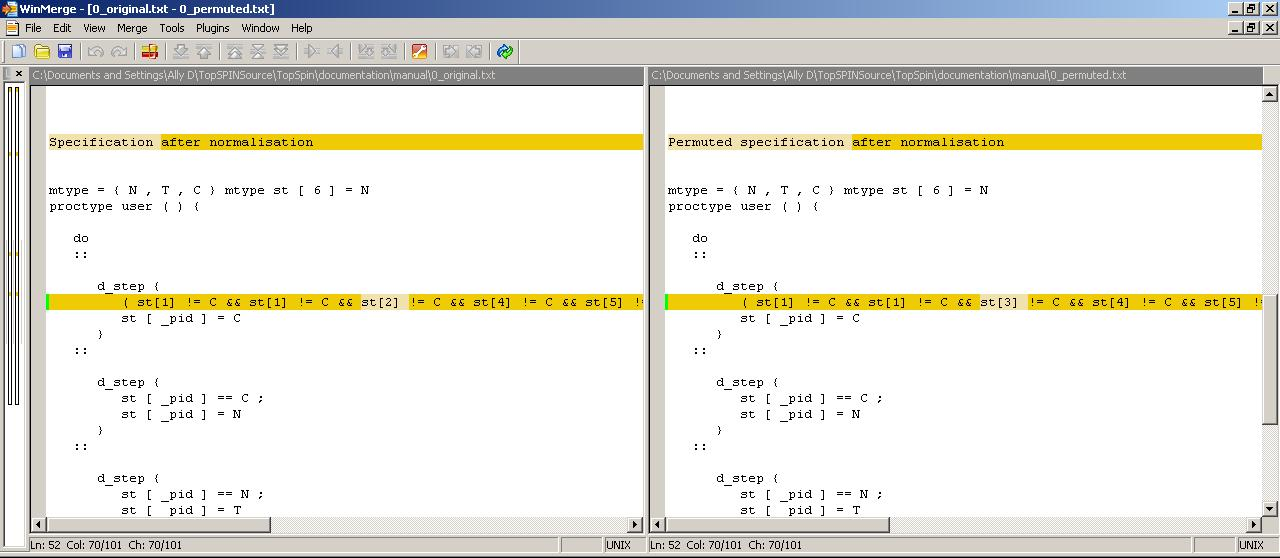
\includegraphics[scale=0.46]{explain.jpg}\caption{Comparing text files output by the \texttt{explain} option to see why symmetry $(3\;2)$ is not valid.}\label{fig:explain}
\end{figure}


\figref{explain} shows the results of comparing these files with WinMerge.  This should alert the user to the fact that the operand \inline{st[1] != C} appears
twice in the highlighted boolean expression: this is clearly a mistake -- one of these operands should be changed to \inline{st[2] != C} to restore full
symmetry and presumably correct the model.

This illustrates the idea that presence of symmetry can actually be a correctness requirement in its own right.

\noindent\textbf{Default value: } 0, \ie no explanations will be given.

\subsection{\texttt{timebound}}

When detecting symmetry, \topspin\ may use a coset search to try to improve upon the initially computed group of symmetries.  This search
can be time-consuming on particular examples.  The \texttt{timebound} integer option limits the length of time dedicated to this search to a maximum
number of seconds.

\noindent\textbf{Default value: } 0, which is used to specify that the coset search should be unbounded.

\subsection{\texttt{conjugates}}

If the coset search is taking a long time, it is sometimes possible to speed things up by picking a number of candidate symmetries
at random, finding the \emph{conjugate} of each known valid generator by these random elements, and then testing the conjugates for
validity.  This is based on the practical observation that valid symmetries are often conjugate to other valid symmetries.  The
\texttt{conjugates} integer option is used to specify how many conjugates to use.

\noindent\textbf{Default value: } 0.  If symmetry detection is slow, try 5 conjugates.

\subsection{\texttt{symmetryfile}}

Sometimes \topspin\ is unable to automatically detect symmetry from an input specification even though the user knows that symmetry exists.
In this case, it is possible to specify a file containing generators for a symmetry group.  The name of this file is specified via the
\texttt{symmetryfile} option.  If \texttt{symmetryfile} is set, \topspin\ will not attempt automatic symmetry detection, and will use the
given group of symmetries for symmetry reduction.

\noindent\textbf{Default value: } no file specified, automatic symmetry detection will be attempted..

\section{Configuration file options for symmetry reduction}\label{sec:overview:symmetryreductionconfig}

\subsection{\texttt{strategy}}

String option specifying the strategy to use for symmetry reduction.  Options are: fast, enumerate, hillclimbing, segment, flatten, exactmarkers, approxmarkers.

\noindent\textbf{Default value: } fast.

\subsection{\texttt{transpositions}}

Boolean option stating whether to apply group elements as transpositions.

\noindent\textbf{Default value: } true.

\subsection{\texttt{stabiliserchain}}

Boolean option stating whether to use a stabiliser chain for enumeration.

\noindent\textbf{Default value: } true.

\subsection{\texttt{vectorise}}

Boolean option stating whether to use vector SIMD instructions for symmetry reduction.  The nature of the resulting
vector code depends on the \texttt{target} configuration file option (see \secref{overview:symmetryreductionconfig:target}).

\noindent\textbf{Default value: } false.

\subsection{\texttt{parallelise}}

Boolean option stating whether to parallelise symmetry reduction using pthreads.

\noindent\textbf{Default value: } false.

\subsection{\texttt{cores}}

Integer option stating the number of cores available for parallel symmetry reduction.

\noindent\textbf{Default value: } 1.

\subsection{\texttt{target}}\label{sec:overview:symmetryreductionconfig:target}

String option specifying the target to use for vector and parallel symmetry reduction.  Options are: PC, CELL, POWERPC.

\noindent\textbf{Default value: } not set by default.

\section{Configuration file options for usability}

\subsection{\texttt{profile}}

Profile the performance of TopSPIN?

\noindent\textbf{Default value: } false.

\subsection{\texttt{verbose}}

Display progress of TopSPIN in detail?

\noindent\textbf{Default value: } false.

\subsection{\texttt{quiet}}

Suppress non-vital output?

\noindent\textbf{Default value: } false.


\chapter{\limitations}\label{chapter:limitations}

Before using \topspin\ for advanced verification it is important to understand
what can and cannot be done with the tool.
\topspin\ places various restrictions on the form a Promela specification may have.
Also, certain \spin\ options are not (yet) compatible with symmetry reduction.

This section briefly described the limitations of \topspin.  Limitations marked
with an asterisk could be removed with relative ease: they just haven't been dealt
with yet.  If you're working with \spin\ and \topspin\ and are being hindered by
these restrictions then please get in tough (\seesec{troubleshooting:gettingintouch}) and efforts will be made
to add appropriate features to \topspin.

\section{Process instantiation and dynamic process creation}

\topspin\ requires all processes to be instantiated using
\inline{run} statements within an \inline{init} process.  The form of the \inline{init}
process must be:

\begin{lstlisting}
init {
  atomic {
     run ...;
     run ...;
     ...
     run ...;
     <other statements>
  }
}
\end{lstlisting}

\noindent \ie all process must be started atomically, and must come before any other statements in the \inline{init}
process (\eg initialisation code), which must also appear within the \inline{atomic} block.

In particular, \topspin\ does \emph{not} support process instantiation using the \inline{active} keyword,
or via \inline{run} statements outside the \inline{init} process.


%
\begin{figure}
\begin{scriptsize}
\begin{verbatim}
proctype P() {

  /* body */

}

proctype Q() {
   ...

   run P();

   ...
}
\end{verbatim}
\end{scriptsize}
\caption{Skeleton Promela specification with dynamic process
creation.}\label{fig:limitations:originaldynamic}
\end{figure}
%
\begin{figure}[t]
\begin{scriptsize}
\begin{verbatim}
chan wakeup_P_1 = [0] of {bit};
chan wakeup_P_2 = [0] of {bit};
chan wakeup_P_3 = [0] of {bit}

proctype P(chan start) {

sleep:
   start?1;

   /* body */

   goto sleep
}

proctype Q() {
   ...

   if :: wakeup_P_1!1
      :: wakeup_P_2!1
      :: wakeup_P_3!1
   fi;

   ...
}

init {
   atomic {
      /* original `run' statements */

      run P(wakeup_P_1);
      run P(wakeup_P_2);
      run P(wakeup_P_3)
   }
}
\end{verbatim}
\end{scriptsize}
\caption{Re-modelled Promela specification without dynamic process
creation.}\label{fig:limitations:remodelleddynamic}
\end{figure}


If a specification relies on dynamic process
creation then it may be possible to re-model the processes as shown
in Figures~\ref{fig:limitations:originaldynamic}
and~\ref{fig:limitations:remodelleddynamic}.
\figref{limitations:originaldynamic} shows a
specification which instantiates copies of proctype $P$ dynamically.
Assuming that 3 is an upper bound for the number of instances of $P$
which should be running at any time,
\figref{limitations:remodelleddynamic} shows an
alternative way of expressing the specification.  The proctype $P$
now includes a channel parameter, and an instance of $P$ waits until
it can receive on this channel before executing its body.  Its body
is identical to the original, except that it includes a final
\inline{goto} statement after which it returns to its initial
configuration.\footnote{This \inline{goto} statement should really
be part of an atomic block which also resets any local variables of
the proctype to their initial values.}  The \inline{init} process
instantiates three copies of $P$, each with a distinct synchronous
channel.  Instead of instantiating a copy of $P$, the proctype $Q$
now offers the literal value 1 to all channels on which instances of
$P$ may be listening.  The example of
Figures~\ref{fig:limitations:originaldynamic}
and~\ref{fig:limitations:remodelleddynamic} can be
adapted to handle multiple process types, with any fixed upper bound
for each process type.



\section{Process termination}\label{sec:limitations:termination}

Technically, process termination destroys symmetry in a Promela specification.  \spin\ only allows processes
to terminate in \emph{reverse} order.  So, if five identical, terminating \texttt{client} proctypes are launched simultaneously
with process identifiers in the range $\{1,2,3,4,5\}$, the processes will terminate one-by-one in a fixed order: 5, 4, 3, 2, 1.
This ordering on process identifiers breaks symmetry between the processes.

Furthermore, the way symmetry reduction is implemented in \topspin\ is not strictly compatible with process termination.  After the
initial state, \topspin\ assumes a fixed set of running processes.  If a process dies, \topspin\ may try to exchange this
processes's state with that of another process when computing symmetry representatives, and this can (very occasionally) lead
to verification-time errors (\seesec{troubleshooting:common:termination}).

If you want to work with terminating processes, you can insert a dummy termination state at the end of each proctype using
a line like the following:

\begin{lstlisting}
end_ok: false
\end{lstlisting}

The \inline{end} label ensures that \spin\ will not complain about instances of the proctype blocking at this label,
and the \inline{false} statement ensures that proctype instances will never truly terminate.

\section{The \protect\inline{_pid} variable should be used}

For symmetry to be detected, it is important for proctypes to use
their built-in \inline{_pid} variable rather than a user-defined
process identifier.  This is illustrated in
Figures~\ref{fig:limitations:originalpid}
and~\ref{fig:limitations:remodelledpid}. Processes in
\figref{limitations:originalpid} are parameterised by a
{\it byte} identifier, which they use to index the \texttt{st}
array. SymmExtractor is not yet sophisticated enough to work out the
correspondence between the \texttt{id} parameter and the built-in
identifier for each process.  However, the specification can be
converted into a form which SymmExtractor can handle, as shown in
\figref{limitations:remodelledpid}. The disadvantage
here is that position 0 of the array \texttt{st} is un-used, meaning
that an array of size three rather than two is required, increasing
the state-vector size by one byte. On the other hand, eliminating
the \texttt{id} variables reduces the state-vector by two bytes, so
the re-modelling works well for this example.

\section{Restrictions on channels$^\ast$}
For simplicity, \topspin\ does not allow channel initialisers to be associated
with channels which are declared locally to a proctype, and does not currently
support arrays of channels.

\begin{figure}
\begin{scriptsize}
\begin{verbatim}
mtype = {N,T,C}
mtype st[2]=N

proctype user(byte id) {
  do
    :: d_step { st[id]==N -> st[id]=T }
    :: d_step { st[id]==T && st[0]!=C && st[1]!=C -> st[id]=C }
    :: d_step { st[id]==C -> st[id]=N }
  od
}

init {
  atomic {
    run user(0);
    run user(1);
  }
}
\end{verbatim}
\end{scriptsize}
\caption{Promela specification which uses user-defined process
identifiers.}\label{fig:limitations:originalpid}
\end{figure}

\begin{figure}
\begin{scriptsize}
\begin{verbatim}
mtype = {N,T,C} mtype st[3]=N;

proctype user() {
  do
    :: d_step { st[_pid]==N -> st[_pid]=T }
    :: d_step { st[_pid]==T && st[1]!=C && st[2]!=C -> st[_pid]=C }
    :: d_step { st[_pid]==C -> st[_pid]=N }
  od
}

init {
  atomic {
    run user();
    run user();
  }
}
\end{verbatim}
\end{scriptsize}
\caption{Re-modelled specification which uses the \protect\inline{_pid}
variable.}\label{fig:limitations:remodelledpid}
\end{figure}

\section{Never claims, trace/notrace constructs, \protect\inline{accept} and \protect\inline{progress} labels}

These are method for specifying liveness properties in a Promela model.  \topspin\ is not
yet compatible with verification of liveness properties, so you will get an error if you try
to apply \topspin\ to a specification containing one of these constructs.

Symmetry \emph{detection} is still possible with liveness verification constructs.  It is OK
to apply \topspin to a specification containing a liveness construct with the \texttt{-detect}
option (\seesec{troubleshooting:gettingintouch}).  The tool will tell you any symmetries it detects; it's just not yet
possible to exploit these symmetries when model checking.

\section{Exclusive send/recieve (\protect\inline{xs}/\protect\inline{xr}) channel assertions}

This is not actually a restriction, rather a warning for users wishing to use these keywords.

Promela includes keywords
\inline{xr} and \inline{xs},
which stand for {\it exclusive receive} and {\it exclusive send}
respectively. A process can include a declaration `\inline{xr}
\emph{name}', where `\emph{name}' is the name of a previously declared
channel, to indicate that only this process can receive messages on
the channel. The \inline{xs} keyword is used similarly.  Providing
\spin\ with this information can lead to more efficient
partial-order reduction. It is not
possible to check, statically, whether \inline{xs} and \inline{xr}
are used correctly, but incorrect uses are flagged by \spin\ during
verification.  These keywords do not affect the presence of symmetry
in the model associated with a specification, so are no problem for
symmetry detection.

However, there is a potential problem with exploiting
\inline{xs}/\inline{xr} information in conjunction with symmetry
reduction, described in Appendix C.1.1 of Donaldson's thesis.  In practice, the
problem with these keywords is unlikely to cause problems: there
is a slim chance that if the keywords are used incorrectly, symmetry reduction
will prevent this from being flagged up during verification.  Therefore, \topspin\
\emph{does} allow these features to be used, but it is the user's responsibility to
use them with care.



\section{Unsigned data type$^\ast$}

Promela supports an \inline{unsigned}
numeric type. A declaration of the form \inline{unsigned} $x$ : $y$
declares an integer variable $x$ which takes non-negative values
which can be represented using $y$ bits.  Clearly the use of this
data type will have no effect on our symmetry detection/reduction
techniques. However, \topspin\ is integrated with an enhanced
Promela type checker which does not currently support the \inline{unsigned}
data type.  A temporary fix for this omission is to replace each occurrence of the
\inline{unsigned} keyword with one of the other numeric types during
symmetry detection.

\section{Sorted send, random receive (\protect\inline{!!} and \protect\inline{??} operators)}

Promela provides alternative channel operators: \inline{!!} (sorted
send) and \inline{??} (random receive).
Sending data on a buffered channel using \inline{!!} causes messages to be queued on the
channel in sorted order. Messages can be retrieved from the buffer
in a random order using \inline{??}. These operators provide a
useful alternative to FIFO channel semantics. They also aid
state-space reduction: storing channel contents in a sorted manner
can be seen as a form of state canonicalisation. However, storing
\inline{pid} messages in a sorted queue imposes an ordering on the set
of process identifiers.  It is not immediately clear whether this
ordering has an effect on symmetry.

For the time being, \topspin\ allows the \inline{!!} and \inline{??} operators to be
used, but they should be used with care.  If you get weird symmetry reduction
results using these operators then please get in touch (\secref{troubleshooting:gettingintouch}).

\section{Embedded C code}

Recent versions of \spin\ allow C code to be embedded in a Promela
specification, and certain variables from the C part of the
specification to be included in the \spin\ state-vector.  Automatic
symmetry detection for this mix of C and Promela is beyond the scope
of \topspin\ at present.


\section{Breadth-first search$^\ast$}

\topspin\ has not been tested with breadth-first search, and will give an
error message if \texttt{sympan.c} is compiled with \texttt{-DBFS}.


\chapter{\buildingfromsource}\label{chapter:compilingfromsource}


\section{Downloading \protect\topspin\ source
code}\label{sec:compilingfromsource:downloading}

The \topspin\ source code is stored in a Subversion repository,
hosted by the Department of Computing Science at the University of
Glasgow at the following URL:
%
\begin{lstlisting}
https://ouen.dcs.gla.ac.uk/repos/symmetry/
\end{lstlisting}
%
Use subversion to check out the \topspin\ source code to an
appropriate location:
%
\begin{lstlisting}
C:\prog>svn checkout https://ouen.dcs.gla.ac.uk/repos/symmetry/trunk TopSPINSource
A TopSPINSource/TestModels
A TopSPINSource/TestModels/EtchTesting
A TopSPINSource/TestModels/EtchTesting/ParsePassTests
A TopSPINSource/TestModels/EtchTesting/ParsePassTests/peterson
A TopSPINSource/TestModels/EtchTesting/ParsePassTests/hello
A TopSPINSource/TestModels/EtchTesting/ParsePassTests/pathfinder
A TopSPINSource/TestModels/EtchTesting/ParsePassTests/snoopy
A TopSPINSource/TestModels/EtchTesting/ParsePassTests/mobile1
A TopSPINSource/TestModels/EtchTesting/ParsePassTests/mobile2
A TopSPINSource/TestModels/EtchTesting/ParsePassTests/pftp
A TopSPINSource/TestModels/EtchTesting/ParsePassTests/leader
A TopSPINSource/TestModels/EtchTesting/ParsePassTests/loops
...
A TopSPINSource/Common/Minimising.gap
A TopSPINSource/Common/parallel_symmetry_cell_ppu.c
A TopSPINSource/Common/Verify.gap
A TopSPINSource/Common/WorkspaceGenerator.gap
A TopSPINSource/Common/parallel_symmetry_cell_spu.c
A TopSPINSource/Common/parallel_symmetry_cell_ppu.h
A TopSPINSource/symmextractor_common_config.txt
Checked out revision 75.
\end{lstlisting}

\section{Generating the Promela parser}\label{sec:compilingfromsource:generating}

\topspin\ is based on a Promela parser which is constructed using
the SableCC parser generator.  Download SableCC version
\sableccversion\ from the Sable
website\footnote{\texttt{\sableccwebsite}}, and generate the parser
as follows (adapting the command according to where you have
installed SableCC):
%
\begin{lstlisting}
java -jar C:\sablecc-3.2\lib\sablecc.jar promela.grammar
\end{lstlisting}
%
This command should result in output similar to the following:
%
\begin{lstlisting}
C:\prog\TopSPINSource>java -jar C:\sablecc-3.2\lib\sablecc.jar
promela.grammar

SableCC version 3.2 Copyright (C) 1997-2003 Etienne M. Gagnon <etienne.gagnon@uqam.ca>
and others.  All rights reserved.

This software comes with ABSOLUTELY NO WARRANTY.  This is free software,
and you are welcome to redistribute it under certain conditions.

Type 'sablecc -license' to view the complete copyright notice and license.

 -- Generating parser for promela.grammar in C:\prog\TopSPINSource
Adding productions and alternative of section AST.
Verifying identifiers.
Verifying ast identifiers.
Adding empty productions and empty alternative transformation if necessary.
Adding productions and alternative transformation if necessary.
computing alternative symbol table identifiers.
Verifying production transform identifiers.
Verifying ast alternatives transform identifiers.
Generating token classes.
Generating production classes.
Generating alternative classes.
Generating analysis classes.
Generating utility classes.
Generating the lexer.
 State: INITIAL
 - Constructing NFA.
..............................................................................
..............................................................................
 - Constructing DFA.
..............................................................................
..............................................................................
 - resolving ACCEPT states.
Generating the parser.
..............................................................................
..............................................................................
\end{lstlisting}

Due to a bug in SableCC, it is then necessary to apply a patch file to the generated parser.  Do this by executing
the following command (you will need to have PERL installed: if you don't, you could easily re-write the
PERL script in your favourite language!).

\begin{lstlisting}
C:\prog\TopSPINSource>perl apply_patch.pl
\end{lstlisting}

\section{Compiling and creating a jar}\label{sec:compilingfromsource:compiling}

You have now downloaded and generated all the Java source code for
\topspin, and can proceed to compile this source code.  The
\inline{javac} compiler and \inline{jar} utility are required to
compile the source and create an executable jar file respectively.
The source code is all contained in directories within \inline{src}.

\subsection{Compiling}

There are two options for compilation:

\begin{enumerate}

\item Create an Eclipse project from the \topspin\ source code, in which case
Eclipse will automatically compile the code.

\item Use the \inline{make} utility and the supplied \inline{Makefile} to compile
the source code, by typing the command \inline{make classes} in the \topspin\
root directory. The provided \inline{Makefile} uses the \inline{sed}
and \inline{find} utilities, which are provided as standard with
Linux, and are available on Windows via Cygwin.

\end{enumerate}
%
Compiling the source code using the \inline{Makefile} gives output
along the following lines:
%
\begin{lstlisting}
C:\prog\TopSPINSource>make classes
javac src/etch/checker/Check.java
Note: .\src\promela\parser\Parser.java uses unchecked or unsafe operations.
Note: Recompile with -Xlint:unchecked for details.
javac src/etch/checker/CheckerTest.java
javac src/etch/testing/EtchTestCase.java
javac src/etch/testing/EtchTester.java
javac src/group/Group.java
javac src/promela/analysis/ReversedDepthFirstAdapter.java
javac src/symmextractor/InlineReplacer.java
javac src/symmextractor/SymmExtractor.java
javac src/symmextractor/testing/SymmExtractorFailTestOutcome.java
javac src/symmextractor/testing/SymmExtractorRunTestOutcome.java
javac src/symmextractor/testing/SymmExtractorTestCase.java
javac src/symmextractor/testing/SymmExtractorTester.java
javac src/symmreducer/testing/ModelCheckingResult.java
javac src/symmreducer/testing/SymmReducerFailTestOutcome.java
javac src/symmreducer/testing/SymmReducerTestCase.java
javac src/symmreducer/testing/SymmReducerTester.java
javac src/testing/RunAllTests.java
\end{lstlisting}
%
Note the compile warnings generated for \inline{Parser.java}: these
are due to code generated by SableCC.  All other files should
compile without warnings.
%
\subsection{Creating a jar file}
%
If you are using Eclipse then you can create an executable jar file
for \topspin\ by exporting your \topspin\ project as a jar, and
selecting \inline{src.TopSpin} as the \emph{main} class.

If using the supplied \inline{Makefile}, typing \inline{make jars}
will produce two jar files:
%
\begin{lstlisting}
C:\prog\TopSPINSource>make jars

jar cmf manifest.txt TopSPIN.jar src/etch/checker/Check.class src/etch/checker/Checker.class
... <many .class files> ...
src/utilities/Strategy.class src/utilities/StringHelper.class src/promela/lexer/lexer.dat
src/promela/parser/parser.dat && echo "TopSPIN.jar built successfully."
TopSPIN.jar built successfully.

jar cmf tests_manifest.txt TopSPINTests.jar src/etch/checker/Check.class
src/etch/checker/Checker.class
... <many .class files> ...
src/utilities/Strategy.class src/utilities/StringHelper.class src/promela/lexer/lexer.dat
src/promela/parser/parser.dat && echo "TopSPINTests.jar built successfully."
TopSPINTests.jar built successfully.
\end{lstlisting}
%
Note that you can skip the \inline{make classes} step, and type
\inline{make jars} to both compile the Java files and produce jar
files.  To delete all jar and class files, use \inline{make clean}.

\section{Try your compiled version on an example}

Now that you have successfully compiled a jar file from the
\topspin\ source, you are effectively in the same position as a user
who has downloaded the \topspin\ jar file using the instructions
given in \secref{downloadandinstall:downloading}.  Of course, you
have the advantage of being able to modify \topspin\ to suit your
purposes!

The next steps involve compiling \saucy, creating a \gap\ workspace,
and testing \topspin\ on a simple example.  Therefore you should
work your way through \chapsref{downloadandinstall}{example}, using
your compiled jar file in place of the downloaded jar file.

\section{Acceptance Tests}\label{sec:compilingfromsource:testing}

The \topspin\ source checkout includes a reasonably large set of
acceptance tests.  It is highly recommended that you run these
tests using the instructions below before commencing any development
work on \topspin\ -- passing the acceptance tests confirms that
you are starting from a stable base.  The acceptance tests can
also be run regularly during development, to ensure that the
addition of new features to \topspin\ does not adversely affect
the tool's existing features.

\vspace{2mm}
\noindent{\bf Important } Before running the acceptance tests, make sure that
the \gcc\ tool is installed in such a way that it can be invoked by
name from a command prompt, i.e. so that typing \inline{gcc} will
launch \gcc. To check this, try typing \inline{gcc} from a fresh
prompt.  You should see something like:
\vspace{2mm}
%
\begin{lstlisting}
C:\>gcc
gcc: no input files
\end{lstlisting}

\subsection{Setting up a configuration file for testing}

The \topspin\ test suite uses a called \inline{symmextractor_common_config.txt}
for some configuration options which apply to most tests.  Open
this file, and edit the \inline{gap} line to use the appropriate command
for your setup.  You should not have to change the \inline{Common} or
\inline{saucy} lines: the source code checkout is organised so that the
\inline{saucy} and \inline{Common} directories are sub-directories of
the directory in which \inline{symmextractor_common_config.txt} is
contained.

\subsection{Running the tests}

You can now run the acceptance
tests via the \inline{TopSPINTests.jar} file:
%
\begin{lstlisting}
java -ea -jar TopSPINTests.jar 2> temp.txt
\end{lstlisting}
%
The \inline{-ea} argument switches on assertion checking, which is useful for
finding potential problems with \topspin.  The final part of the command,
\inline{2> temp.txt}, pipes error messages generated during testing to the
file \inline{temp.txt}.  This is useful since many of the tests are
\emph{fail} tests, which check that the \topspin\ typechecker correctly
rejects Promela specifications which are not suitable for processing by
\topspin.  Redirecting these error messages to a text file means that
the screen is not cluttered with error messages.

You should see something like this when you run the tests:
%
\begin{lstlisting}
ETCH TESTS
==========
   [PASS] expected and actual: BadlyTyped, file: TestModels/EtchTesting/FailTests/failrec...
   [PASS] expected and actual: WellTyped, file: TestModels/EtchTesting/PassTests/testtele...
   [PASS] expected and actual: WellTyped, file: TestModels/EtchTesting/PassTests/test_ex_...
   [PASS] expected and actual: WellTyped, file: TestModels/EtchTesting/PassTests/testtele...
   [PASS] expected and actual: BadlyTyped, file: TestModels/EtchTesting/FailTests/faildup...
   [PASS] expected and actual: ParsePass, file: TestModels/EtchTesting/ParsePassTests/pet...
   ...


SYMMEXTRACTOR TESTS
===================
   [PASS] expected and actual: (well typed, group size = 72, coset search: no), file: Tes...
   [PASS] expected and actual: (well typed, group size = 1296, coset search: no), file: T...
   [PASS] expected and actual: BreaksRestrictions, file: TestModels/SymmExtractorTests/Ba...
   [PASS] expected and actual: (well typed, group size = 3628800, coset search: no), file...
   [PASS] expected and actual: BreaksRestrictions, file: TestModels/SymmExtractorTests/Ba...
   ...


SYMMREDUCER TESTS
=================
   [PASS] expected and actual: ((well typed, group size = 120, coset search: no), no. sta...
   [PASS] expected and actual: ((well typed, group size = 3628800, coset search: no), no....
   [PASS] expected and actual: ((well typed, group size = 6, coset search: no), no. state...
   [PASS] expected and actual: ((well typed, group size = 5040, coset search: no), no. st...
   [PASS] expected and actual: ((well typed, group size = 720, coset search: no), no. sta...
   ...


Summary:
   238 passes
   0 fails


Acceptance tests passed - you may commit your changes!
\end{lstlisting}
%
There are in the order of 250 test cases.  These are divided into
\etch\ tests, which test the typechecking component of \topspin;
\symmextractor\ tests, which check the symmetry detection
capabilities of the tool, and \symmreducer\
tests, which perform symmetry reduction on Promela examples, checking
that verification results for these examples are as expected.
The \etch\ tests run very quickly, the \symmextractor\ tests run
at a moderate speed, and the \symmreducer\ tests run fairly slowly.
Testing takes approximately 10 minutes on an average PC.

\subsection{Problems running the tests}

If you have compiled a fresh checkout of \topspin\ then all of the acceptance
tests should pass, since their passing is a condition for committing
changes to the source code repository.  Therefore, if you have any problems
running the tests this is likely due to a problem with the way you have
set up \gap, \saucy, \spin, or \gcc.  Have a look at \secref{troubleshooting:common}
which details common problems encountered when using \topspin.  If test
cases continue to fail then please send a bug report to the \topspin\
development team: see \secref{troubleshooting:reportingbugs} for details.


\chapter{\troubleshooting}\label{chapter:troubleshooting}

This section includes a list of common problems with the use of \topspin.
Please also refer to current limitations of \topspin, in \chapref{limitations}.

\section{Common problems}\label{sec:troubleshooting:common}

%%%%%%%%%%%%%%%%%%%%%%%%%%%%%%%

\subsection{Missing configuration file}

\problem{There is no file named \inline{config.txt} in your working
directory when you run \topspin.}

\exampleerrormessage

\begin{lstlisting}
Error opening configuration file "config.txt", which should be
located in the directory from which you run TopSPIN.
\end{lstlisting}

\solution{Follow the instructions in \secref{example:configuration}
on how to create \inline{config.txt}.}

%%%%%%%%%%%%%%%%%%%%%%%%%%%%%%%

\subsection{Incomplete configuration file}

\problem{The file \inline{config.txt} does not contain entries for all of the
mandatory options, \inline{gap}, \inline{saucy} and \inline{common}.}

\exampleerrormessage

\begin{lstlisting}
No configuration specified for GAP.
No configuration specified for saucy.
No common directory specified.
\end{lstlisting}

\solution{Follow the instructions in \secref{example:configuration}
on how to create \inline{config.txt} with these mandatory options.}

%%%%%%%%%%%%%%%%%%%%%%%%%%%%%%%

\subsection{The \saucy\ program is not correctly installed}

\problem{You may not have correctly installed and compiled \saucy,
the graph automorphism program on which \topspin\ relies.}

\exampleerrormessage

\begin{lstlisting}
Error launching saucy with command: C:\Program Files\TopSPIN\saucy\saucy.exe -d
"C:\Program Files\TopSPIN\Common\graph.saucy"
java.io.IOException: CreateProcess: C:\Program Files\TopSPIN\saucy\saucy.exe -d
"C:\Program Files\TopSPIN\Common\graph.saucy" error=2
        at java.lang.ProcessImpl.create(Native Method)
        ... rest of Java stack trace
\end{lstlisting}

\solution{Source code for \saucy\ is included with the \topspin\
distribution, which can be downloaded via the instructions of
\secref{downloadandinstall:downloading}.  However, you need to
compile the \saucy\ source code using \gcc. To do this, follow the
instructions given in
\secref{downloadandinstall:installation:compilingsaucy}.}

%%%%%%%%%%%%%%%%%%%%%%%%%%%%%%%

\subsection{Path to \saucy\ in configuration file is wrong}

\problem{From \topspin's point of view this is the same as the
previous problem.  From your point of view there is a difference:
you may have correctly installed and compiled \saucy, but but
mistyped the path to \saucy\ in \inline{config.txt}.}

\exampleerrormessage

\begin{lstlisting}
Error launching saucy with command: C:\Program Files\TopSPIN\saucy\tsaucy.exe -d
"C:\Program Files\TopSPIN\Common\graph.saucy"
java.io.IOException: CreateProcess: C:\Program Files\TopSPIN\saucy\tsaucy.exe -d
"C:\Program Files\TopSPIN\Common\graph.saucy" error=2
        at java.lang.ProcessImpl.create(Native Method)
        ... rest of Java stack trace
\end{lstlisting}
%
Note that \topspin\ is trying to launch \inline{tsaucy.exe} rather
than \inline{saucy.exe}, due to a typo in \inline{config.txt}.

\solution{Make sure \saucy\ is correctly downloaded and compiled
(\secref{downloadandinstall:installation:compilingsaucy}), and
ensure that \inline{config.txt} contains a line for \saucy\ with
\emph{exactly} the absolute path to the tool
(\secref{example:configuration}).}

%%%%%%%%%%%%%%%%%%%%%%%%%%%%%%%

\subsection{\protect\gap\ is not correctly installed}

\problem{You may not have correctly installed \gap, the
computational group theory package on which \topspin\ relies.}

\exampleerrormessage

\begin{lstlisting}
Starting GAP with command: C:\gap4r4\bin\gap.bat -L
"C:\Program Files\TopSPIN\Common\gapworkspace" -q
Exception in thread "main"
java.io.IOException: CreateProcess: C:\gap4r4\bin\gap.bat -L
"C:\Program Files\TopSPIN\Common\gapworkspace" -q error=2
        at java.lang.ProcessImpl.create(Native Method)
        ... rest of Java stack trace
\end{lstlisting}

\solution{Download and install \gap\ from the \gap\ website.  The
URL for this website and the version of \gap\ which \topspin\
supports are given in \figref{symmextractorandtopspin:prerequisites}
(\secref{downloadandinstall:prerequisites}).}

%%%%%%%%%%%%%%%%%%%%%%%%%%%%%%%

\subsection{Path to \protect\gap\ in configuration file is wrong}

\problem{From \topspin's point of view this is the same as the
previous problem.  From your point of view there is a difference:
you may have correctly installed \gap, but mistyped the path to
\gap\ in \inline{config.txt}.}

\exampleerrormessage

\begin{lstlisting}
Starting GAP with command: C:\gap4r4\bin\tgap.bat -L
"C:\Program Files\TopSPIN\Common\gapworkspace" -q
Exception in thread "main"
java.io.IOException: CreateProcess: C:\gap4r4\bin\tgap.bat -L
"C:\Program Files\TopSPIN\Common\gapworkspace" -q error=2
        at java.lang.ProcessImpl.create(Native Method)
        ... rest of Java stack trace
\end{lstlisting}
%
Note that \topspin\ is trying to launch \inline{tgap.bat} rather
than \inline{gap.bat}, due to a typo in \inline{config.txt}.

\solution{Make sure you have correctly downloaded and installed \gap
(\secref{downloadandinstall:prerequisites}), and ensure that
\inline{config.txt} contains a line for \gap\ with \emph{exactly}
the absolute path to the tool (\secref{example:configuration}).}

%%%%%%%%%%%%%%%%%%%%%%%%%%%%%%%

\subsection{Common directory does not exist, or user does not have permissions for this directory}

\problem{The location of the \topspin\ \inline{Common} directory has
been specified incorrectly in \inline{commmon.txt}.}

\exampleerrormessage

\begin{lstlisting}
Error while trying to create file "C:\Program Files\TopSPIN\Common\graph.saucy".
Make sure that the directory C:\Program Files\TopSPIN\Common\ exists,
and that you have write permission.
\end{lstlisting}

\solution{Make sure that \inline{config.txt} contains a line of the
form \inline{common=}\emph{name}, where \emph{name} is the
\emph{absolute} path to the \inline{Common} directory provided with
the \topspin\ distribution.  Make sure this path has not been
mistyped, and that the path includes a terminating slash.}

%%%%%%%%%%%%%%%%%%%%%%%%%%%%%%%

\subsection{Path to Common directory does not have terminating slash}

\problem{The location of the \topspin\ \inline{Common} directory has
been specified without a final forward- (Linux) or back- (Windows) slash.}

\exampleerrormessage

\begin{lstlisting}

\end{lstlisting}

\solution{Make sure that \inline{config.txt} contains a line of the
form \inline{common=}\emph{name}, where \emph{name} is the
\emph{absolute} path to the \inline{Common} directory provided with
the \topspin\ distribution.  Make sure this path has not been
mistyped, and that the path includes a terminating slash.}

%%%%%%%%%%%%%%%%%%%%%%%%%%%%%%%

\subsection{Missing or corrupt \protect\gap\ workspace}

\problem{The file \inline{gapworkspace} in the \inline{Common}
directory is either missing or corrupted.}

\exampleerrormessage

\begin{lstlisting}
Starting GAP with command: C:\gap4r4\bin\gap.bat -L
"C:\Program Files\TopSPIN\Common\gapworkspace" -q
Error -- bad GAP workspace specified in configuration file.

GAP produced errors:
====================
gap: Press <Enter> to end program
End of GAP errors
\end{lstlisting}

\solution{Check that:
%
\begin{enumerate}
\item You have followed the instructions in \secref{downloadandinstall:gapworkspace} on creating a \gap\ workspace
\item This workspace has been successfully saved in the \inline{Common} directory
\item You have not changed the version of \gap\ you are using since creating the workspace
\item The workspace was created exactly the same machine, with the same operating system,
on which you are running \topspin.
\end{enumerate}
}

%%%%%%%%%%%%%%%%%%%%%%%%%%%%%%%

\subsection{\protect\gap\ executable specified in configuration file, instead of shell script/batch file}

\problem{You have specified the path to the \gap\ executable as the \inline{gap} option in \inline{config.txt}.}

\exampleerrormessage

\begin{lstlisting}
GAP produced errors:
====================
Error, the library file 'system.g' must exist and be readable called from
CallFuncList( func, arg ); called from
RereadLib( "system.g" ); called from
<function>( <arguments> ) called from read-eval-loop
Entering break read-eval-print loop ...
you can 'quit;' to quit to outer loop, or
you can 'return;' to continue
brk>
\end{lstlisting}

\solution{Open \inline{config.txt} and change the \inline{gap} option to refer to the shell script
(\inline{gap.sh}) or batch file (\inline{gap.bat}).}

%%%%%%%%%%%%%%%%%%%%%%%%%%%%%%%

\subsection{\protect\spin\ is not correctly installed}

\problem{You have not correctly installed \spin\ in such a way that
the tool can be invoked by simply typing \inline{spin}, as discussed
in \secref{downloadandinstall:prerequisites}.}

\exampleerrormessage

\begin{lstlisting}
An error occurred while constructing the "sympan" files.
java.io.IOException: CreateProcess: spin -a loadbalancer.p error=2
        at java.lang.ProcessImpl.create(Native Method)
        ... rest of Java stack trace
\end{lstlisting}

\solution{Make sure \spin\ is correctly installed, and that the
directory containing the \spin\ executable is part of your
\emph{path} environment variable.  Perhaps you have
renamed \inline{spin} to \inline{spin-linux} or \inline{spin516};
maybe you do not have execute permission for \spin, or perhaps you
have another application called \inline{spin} installed on your
machine. Resolve these issues so that \inline{spin} is all that
needs to be typed to launch the \spin\ tool.}

%%%%%%%%%%%%%%%%%%%%%%%%%%%%%%%

\subsection{C preprocessor, \protect\inline{cpp}, unavailable}

\problem{\topspin\ uses the \inline{cpp} program to expand \inline{#define} and \inline{#include}
macros before processing a specification.  If \inline{cpp} is not available then \topspin\ can
still be invoked, but cannot handle specifications which include these directives.}

\exampleerrormessage

\begin{lstlisting}
C preprocessor (cpp) not available - TopSPIN will not work correctly on files which use
#define or #include.
src.promela.lexer.LexerException: [1,1] Unknown token: #
    ... rest of Java stack trace
\end{lstlisting}

\solution{Install the \inline{cpp} program on your system.  Linux distributions provide
\inline{cpp} as standard; under Windows the \inline{cpp} program is provided as part of
Cygwin.  Make sure \inline{cpp} is in your path.}

%%%%%%%%%%%%%%%%%%%%%%%%%%%%%%%

\subsection{Typechecking error: problem with array index}

\problem{By default, \topspin\ performs strict typechecking and only allows arrays to be accessed using \texttt{byte} or \texttt{pid} types.}

\exampleerrormessage

\begin{lstlisting}
Error at line 8: Type "int" cannot be used as an array index, it is not a subtype of "byte".
\end{lstlisting}

\solution{You can use the \texttt{-relaxedarrayindexing} option to make this error go away (see \secref{overview:commandline:relaxedarray}), or refactor your specification so
that arrays are indeed only indexed by \texttt{byte} or \texttt{pid} expressions: this may make the associated state-vector smaller.}

%%%%%%%%%%%%%%%%%%%%%%%%%%%%%%%

\subsection{Typechecking error: problem with assignment to numeric variable}

\problem{By default, \topspin\ performs strict typechecking and only allows a variable to be assigned a value of a ``smaller'' type, \eg assignment of
\texttt{byte} to \texttt{short} is OK, but not the other way round.  Sometimes this is too restrictive.}

\exampleerrormessage

\begin{lstlisting}
Error at line 8: invalid assignment -- Type "short" occurs in a context where it is required to be a subtype of "byte".
\end{lstlisting}

\solution{You can use the \texttt{-relaxedassignment} option to make this error go away (see \secref{overview:commandline:relaxedassign}),
or refactor your specification so that assignments to numeric variables are always from expressions with a smaller type: this may make the
associated state-vector more compact.}

%%%%%%%%%%%%%%%%%%%%%%%%%%%%%%%

\subsection{Error during verification: ``bad proctype''}\label{sec:troubleshooting:common:termination}

\problem{Verification quits with a ``bad proctype'' error message.}

\exampleerrormessage

\begin{lstlisting}
pan: bad proctype - collapse (at depth 1023)
\end{lstlisting}

\solution{This error can occur if your specification involves proctypes which terminate.  See \secref{limitations:termination} for details of this, and for a technique
to prevent \spin\ processes from terminating by providing an inescapable final state.  This error message will only be generated if
\texttt{COLLAPSE} compression is used.  Nevertheless, for reasons explained in \secref{limitations:termination} it is best to apply \topspin\ to systems of non-terminating
processes.}


%%%%%%%%%%%%%%%%%%%%%%%%%%%%%%%


%\subsection{}
%
%\problem{}
%
%\exampleerrormessage
%
%\begin{lstlisting}
%\end{lstlisting}
%
%\solution{}

%
\section{Reporting bugs in \protect\topspin}\label{sec:troubleshooting:reportingbugs}
%
If you have a problem using \topspin, first check to see if your
problem is covered by one of the \emph{common problems} in
\secref{troubleshooting:common}.  If this is not the case, then
please take the time to report your bug to the \topspin\ developers,
so that it can be immediately documented and ultimately fixed, for
the benefit of you and other \topspin\ users.

Bug reports should be submitted using the contact details in
\secref{troubleshooting:gettingintouch}.  Please provide the
following when reporting a bug:

\begin{itemize}
\item A description of the problem
\item A test-case (example Promela specification and \inline{config.txt} file) which exposes the problem
\item The \topspin\ version you are using, the approximate date on which you downloaded \topspin
\item Details as to whether you are using a pre-compiled version of \topspin, or a version you have compiled from source
\item Any ideas you have as to what may have gone wrong!
\end{itemize}

Please note that bugs do not have to relate to the correctness of
\topspin\ -- a valuable bug report could be in response to a
misleading error message generated by \topspin, where there
\emph{is} something wrong with the input specification, but the
problem is not what the error message indicates.  Please feel free
to also submit suggestions for features to be added to \topspin.

\section{Reporting bugs in this manual}

Please also get in touch (\secref{troubleshooting:gettingintouch})
if you find typos, inconsistencies or ambiguities in this manual --
this kind of feedback is extremely valuable.

\section{Getting in touch}\label{sec:troubleshooting:gettingintouch}

All correspondence related to \topspin\ should be by email, to
Alastair Donaldson: \inline{ally@codeplay.com}.


\chapter*{Acknowledgements}

\begin{itemize}

\item \topspin\ was originally developed by Alastair Donaldson at the University of Glasgow, between 2003 and 2006.

\item \topspin\ uses symmetry reduction theory developed by Alastair Donaldson and Alice Miller.  This theory is
in turn based on a decade of research by the model-checking
community.

\item Thanks to the following people for reporting bugs in \topspin, and feedback on the instructions in this
manual: Silver Juurik, Jan Rakow, Shamim Rippon, Iryna Shkvarko.

\item Thanks to Gerard Holzmann, designer of \spin, for advice on integrating symmetry reduction with other \spin\ state-space reduction techniques.

\item The approach taken by the \topspin\ implementation was influenced greatly by the SymmSpin tool, developed
by Dragan Bosnacki, Denis Dams and Lezek Holenderski.

\item The manual layout was inspired by the \gap\ reference manual.

\item Thanks to the developers of \gap, \saucy\ and SableCC: the development of \topspin\ would have taken a lot
longer without these excellent tools.

\end{itemize}


\end{document}
